\begin{questions}
	\section{Exercise 1: Implement a “Safe Waypoint Navigation” Action.}

	\subsection{Adding a vehicle position control objective}
	\question
	Initialize the vehicle far away from the seafloor. An example position could be

	\begin{displaymath}
		\vec{p}
		=
		\begin{bmatrix}
			10.5 & 35.5 & -36 & 0 & 0 & \pi/2
		\end{bmatrix}\T
	\end{displaymath}
	Give a target position that is also sufficiently away from the seafloor, e.g.,
	
	\begin{displaymath}
		\vec{vehicleGoalPosition}
		=
		\begin{bmatrix}
			10.5 & 37.5 & -38 & 0 & 0 & 0
		\end{bmatrix}\T
	\end{displaymath}

	Goal: Implement a vehicle position control task, and test that the vehicle
	reaches the required position and orientation.

	\begin{parts}
		\part{What is the Jacobian relationship for the Vehicle Position control task? How was the task reference computed?}
		\begin{solutionorbox}
			Let $\xdot = \J\ydot$ be the Jacobian relationship
			between the task variables, and the control variables.
			We remind ourselves that the control variables vector is
			defined such that
			\[
				\ydot =
				\begin{bmatrix}
					\qdot\quad
					\vl[v]\quad
					\va[v]
				\end{bmatrix}\T
				\mathrm{,}
			\]
			where $\qdot\in\Rnm17$, $\vl[v],\va[v]\in\Rnm13$.

			The Vehicle Position control task computes the control
			variables separately for linear and angular velocities.

			Thus, the jacobians for the Vehicle Position control task are
			\begin{align*}
				&\J[w]_{\vl} =
				\begin{bmatrix}
					\Znm37\quad
					\Rot{w}{v}\quad
					\Znm33
				\end{bmatrix}\\
				&\J[w]_{\va} =
				\begin{bmatrix}
					\Znm37\quad
					\Znm33\quad
					\Rot{w}{v}
				\end{bmatrix}
				\mathrm{.}
			\end{align*}
			
			The references rates $\xdotbar{\vl}$ and
			$\xdotbar{\va}$ are defined as
			\begin{align*}
				&\xdotbar[w]{\vl} =
				\lambda\left(\Rot[\mathrm{goal}]{w}{v} -
				\Rot{w}{v}\right)
				\\
				&\xdotbar[w]{\va} =
				\lambda\left(\mathrm{VersorLemma}(\Rot[\mathrm{goal}]{w}{v},
				\Rot{w}{v})\right)
				\\
				&\lambda\in\mathbb{R}^+
				\mathrm{,}
			\end{align*}

			where VersorLemma is a function computing the
			misalignement vector between two orientations matrixes
			by using the unit vector lemma and $\lambda$ is a
			positive arbitrary real.

			Both references rates are then saturated.

		\end{solutionorbox}
		\part{What is the behaviour if the Horizontal Attitude is enabled
			or not? Try changing the initial or target orientation in terms of roll and
		pitch angles. Discuss the behaviour.}

		\begin{solutionorbox}
			For the given initialization, the Horizontal Attitude
			task did not activate. We modified the target
			orientation to $\left(0, -\frac{\pi}{2}, 0\right)$.

			Enabling the Horizontal Attitude task with a higher
			priority than the Vehicle Position task (for angular
			velocities) severely restricts the manifold of solutions
			computed. The restriction is illustrated in
			Figure~\ref{fig:ex1_ha}, where the task is disabled,
			then enabled for the same orientation goal.

			Without the Horizontal Attitude task, the vehicle
			successfully orients itself according to the goal, as
			demonstrated in Figure~\ref{subfig:ex1_ha_disabled}.

			With the Horizontal Attitude task enabled however, the
			vehicle seems to be stuck in a compromise between the
			two tasks where neither one is fully satisfied, as seen
			in Figure~\ref{subfig:ex1_ha_enabled}. The reason being,
			higher priority tasks partially fix the control
			variables, such that subsequent tasks only optimize the
			remaining arbitrariness and not the control variables
			themselves. In practice, that leads the lower priority
			tasks to be considered as a preference as not a
			requirement.
		\end{solutionorbox}
		\begin{figure}
			\begin{subfigure}[b]{0.5\linewidth}
				\centering
				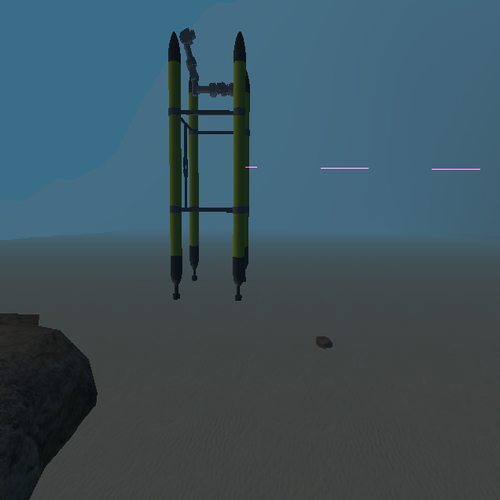
\includegraphics[width=\linewidth]{ex1_ha_disabled.png}
				\caption{Horizontal Attitude disabled}%
				\label{subfig:ex1_ha_disabled}
			\end{subfigure}%
			\begin{subfigure}[b]{0.5\linewidth}
				\centering
				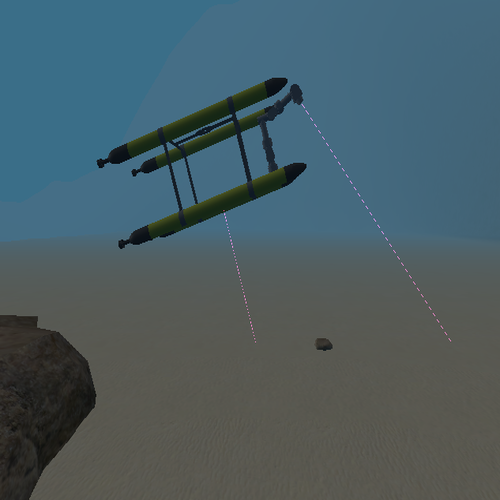
\includegraphics[width=\linewidth]{ex1_ha_enabled.png}
				\caption{Horizontal Attitude
				enabled}%
				\label{subfig:ex1_ha_enabled}
			\end{subfigure}

			\caption{Vehicle angular velocities (Goal
			orientation $\left(0, -\frac{\pi}{2}, 0\right)$)}%
			\label{fig:ex1_ha}
		\end{figure}


		\part{Swap the priorities between Horizontal Attitude and the
		Vehicle Position control task. Discuss the behaviour.}
		\begin{solutionorbox}
			When exchanging priorities, the Vehicle Position control
			task is always enabled, as it has the highest priority.

			The behaviour is similar to the previous situation,
			where the Horizontal Attitude task was disabled (see
			Figure~\ref{subfig:ex1_ha_disabled}), the Vehicle
			Position control task is fully satisfied, while the
			Horizontal Attitude task is never satisfied.

			Previously, when both tasks were activated but their
			priorities reversed, both tasks were partially
			satisfied. However, in the situation where the Vehicle
			Position control task has a higher priority, then it
			supersedes the Horizontal Attitude task.

			Probably, the manifold of solutions first computed by
			the Horizontal Attitude task has considerably more
			leeway in terms of optimization, which leads the
			subsequent task to be partially fulfilled. The Vehicle
			Position control task does not have the same leeway,
			which leads to its dominance.
		\end{solutionorbox}
	\end{parts}

	\subsection{Adding a safety minimum altitude control objective}
	\question
	Initialize the vehicle at the position:

	\begin{displaymath}
		\vec{p}
		=
		\begin{bmatrix}
			48.5 & 11.5 & -33 & 0 & 0 &-\pi/2
		\end{bmatrix}\T
	\end{displaymath}

	Choose as target point for the vehicle position the following one:

	\begin{displaymath}
		\vec{vehicleGoalPosition}
		=
		\begin{bmatrix}
			50 & -12.5 & -33 & 0 & 0 & -\pi/2
		\end{bmatrix}\T
	\end{displaymath}
	Goal: Implement a task to control the altitude from the seafloor. Check that at
	all times the minimum distance from the seafloor is guaranteed.

	\begin{parts}
		\part{Report the new hierarchy of tasks of the Safe Waypoint
			Navigation and their priorities. Comment how you choose the priority level for
		the minimum altitude.}

		\begin{solutionorbox}
			The hierarchy of tasks for the Safe Waypoint Navigation
			is described in
			Table~\ref{table:tkip_safe_waypoint_navigation_robust}, where
			the minimum altitude task has the highest priority.

			During the Safe Waypoint Navigation, the minimum
			altitude task must be activated whenever necessary, that
			is when the vehicle's altitude goes over an arbitrary
			threshold. When activated, its directives must
			supersede other possibly conflicting tasks, otherwise
			the vehicle might accidentally collide with the ground,
			which is undesired.
		\end{solutionorbox}
		\begin{table}[htb]
			\caption{Hierarchy of tasks for Safe Waypoint Navigation
			- ROBUST }
			\label{table:tkip_safe_waypoint_navigation_robust}
			\begin{center}
				\footnotesize
				\begin{tabular}{ccccc}
					\toprule
					Task & Type & Safe Waypoint Navigation
					\\
					\midrule
					Minimum altitude & I & 1 \\
					\hdashline
					Horizontal attitude & I & 2 \\
					\hdashline
					Vehicle position & I & 3 \\
					\bottomrule
				\end{tabular}
			\end{center}
		\end{table}%


		\part{What is the Jacobian relationship for the Minimum Attitude
			control task? Report the formula for the desired task reference generation, and
		the activation thresholds.}

		\begin{solutionorbox}
			We consider the actual vehicle altitude $a$, and the
			distance vector given by the sensor \vect{d}. Let \vect[v]{n} be the
			seafloor normal vector projected on the vehicle frame
			\cframe v.
			The vehicle altitude is considered as \[
				a = \vec[v]n\cdot\vec[v]d\mathrm{,}
			\] where the vector
			\vect d is projected on the vehicle frame.

			Consequently, if we assume the seafloor is flat, then we
			can write that \[
				\dot a = \vec[v]n\cdot\vec{v}_{v/w}\mathrm{,}
			\] where $\vec{v}_{v/w}$ is the linear
			velocity vector of the vehicle frame \cframe{v} with
			respect to the world frame \cframe{w}.

			Thus, we can write the jacobian for the minimum
			altitude control task, that is \[
				\J[v]_{\ma} = \begin{bmatrix}
					\Znm17\quad
					\vec[v]n\T\quad
					\Znm13
				\end{bmatrix}\mathrm{.}
			\]

			The desired task reference is generated using the
			following formula \[
				\xdotbar[v]{\ma} = \lambda(\ma - \vec{a}) +
				1\quad \lambda\in\mathbb{R}^+
				\mathrm{.}
			\]

			We introduce a bias of $1$, to prevent the reference
			rate from converging to small values. Indeed, when the
			vehicle altitude is close to its objective, the
			reference rate might become insignificant, which might
			endanger the vehicle's safety, as the task can be fully
			activated whilst not influencing the control variables
			to the full extent it ought to.

			The activation thresholds are $\left[\vec{ma};
			\vec{ma} + 0.5\right]$. If the minimum altitude
			requirement must be very strict, then a safety buffer
			can be added to the interval, as to activate the task
			earlier.

		\end{solutionorbox}

		\part{Try imposing a minimum altitude of 1, 5, 10 m respectively.
		What is the behaviour? Does the vehicle reach its final goal in all cases?}

		\begin{solutionorbox}
			For the 1 m minimum altitude task, the vehicle
			successfully arrives at its goal destination, whilst
			doing its best to respect the minimum altitude task.
			When 5 or 10 m is imposed, the minimum altitude task
			conflicts with the vehicle position task and the latter
			is superseded in terms of altitude due to the priorities.

			If the imposed minimum altitude is 1 m, then the vehicle
			immediately moves towards its goal, as the minimum
			altitude task is not activated in the first few seconds.

			If the imposed minimum altitude is either 5 or 10 m,
			then the minimum altitude task is immediately activated,
			leading to the vehicle increasing its altitude until the
			minimum altitude has been reached. Other active tasks
			run in parallel.
		\end{solutionorbox}

		\part{How was the sensor distance processed to obtain the altitude
			measurement? Does it work in all cases or some underlying assumptions are
		implicitly made?}

		\begin{solutionorbox}
			The altitude measurement is obtained by the dot product
			of the seafloor normal vector and the sensor distance
			\vect d. This method does not work in all cases, as the
			sensor could point towards an irregular seafloor. That
			is, if the vehicle is above a slope and/or tilted, then the
			process could either return a lower or higher altitude
			than expected.
		\end{solutionorbox}
	\end{parts}
